%%%%%%%%%%%%%%%%%%%%%%%%%%%%%%%%%%%%%%%%%
%  My documentation report
%  Objective: Explain what I did and how, in order to help someone continue with the investigation
%
% Important note:
% Chapter heading images should have a 2:1 width:height ratio,
% e.g. 920px width and 460px height.
%
% The images can be found anywhere, usually on sky surveys websites or the
% Astronomy Picture of the day archive http://apod.nasa.gov/apod/archivepix.html
%
% The original template (the Legrand Orange Book Template) can be found here --> http://www.latextemplates.com/template/the-legrand-orange-book
%
% Original author of the Legrand Orange Book Template:
% Mathias Legrand (legrand.mathias@gmail.com) with modifications by:
% Vel (vel@latextemplates.com)
%
% Original License:
% CC BY-NC-SA 3.0 (http://creativecommons.org/licenses/by-nc-sa/3.0/)
%%%%%%%%%%%%%%%%%%%%%%%%%%%%%%%%%%%%%%%%%
 
%----------------------------------------------------------------------------------------
%	PACKAGES AND OTHER DOCUMENT CONFIGURATIONS
%----------------------------------------------------------------------------------------

\documentclass[11pt,fleqn,english,russian]{report} % book or report

\usepackage[top=3cm,bottom=3cm,left=3.2cm,right=3.2cm,headsep=10pt,letterpaper]{geometry} % Page margins

\usepackage{hyperref}
\usepackage{courier}
\usepackage{xcolor} % Required for specifying colors by name
\definecolor{ocre}{RGB}{25,50,150} % Define the orange color used for highlighting throughout the book

\definecolor{tssteelblue}{RGB}{70,130,180}
\definecolor{tsorange}{RGB}{255,138,88}
\definecolor{tsblue}{RGB}{23,74,117}
\definecolor{tsforestgreen}{RGB}{21,122,81}
\definecolor{tsyellow}{RGB}{255,185,88}
\definecolor{tsgrey}{RGB}{200,200,200}

\definecolor{codegreen}{rgb}{0,0.6,0}
\definecolor{codegray}{rgb}{0.5,0.5,0.5}
\definecolor{codepurple}{rgb}{0.58,0,0.82}
\definecolor{backcolour}{rgb}{0.95,0.95,0.92}

\usepackage{listings}
%Code listing style named "mystyle"
\lstdefinestyle{mystyle}{
	backgroundcolor=\color{tsblue!10},   commentstyle=\color{codegreen},
	keywordstyle=\color{magenta},
	numberstyle=\tiny\color{codegray},
	stringstyle=\color{codepurple},
	basicstyle=\ttfamily\footnotesize,
	breakatwhitespace=false,         
	breaklines=true,                 
	captionpos=b, 
	xleftmargin=.05\linewidth,
	keepspaces=true,                 
	numbers=left,                    
	numbersep=5pt,                  
	showspaces=false,                
	showstringspaces=false,
	showtabs=false,                  
	tabsize=2
}

\usepackage{listings}
\lstset{basicstyle=\footnotesize\ttfamily,breaklines=true, style=mystyle}
\lstset{framextopmargin=50pt,frame=bottomline}

\usepackage{graphicx}

% Font Settings
\usepackage{avant} % Use the Avantgarde font for headings
%\usepackage{times} % Use the Times font for headings
\usepackage{mathptmx} % Use the Adobe Times Roman as the default text font together with math symbols from the Sym­bol, Chancery and Com­puter Modern fonts

\usepackage{microtype} % Slightly tweak font spacing for aesthetics
\usepackage[utf8]{inputenc} % Required for including letters with accents
\usepackage[T2A]{fontenc}

% Bibliography
%\usepackage[style=alphabetic,sorting=nyt,sortcites=true,autopunct=true,babel=hyphen,hyperref=true,abbreviate=false,backref=true,backend=biber]{biblatex}
%\addbibresource{bibliography.bib} % BibTeX bibliography file
%\defbibheading{bibempty}{}

%%%%%%%%%%%%%%%%%%%%%%%%%%%%%%%%%%%%%%%%%
% This is based on the Legrand Orange Book
% Structural Definitions File
%
% The original template (the Legrand Orange Book Template) can be found here --> http://www.latextemplates.com/template/the-legrand-orange-book
%
% Original author of the Legrand Orange Book Template::
% Mathias Legrand (legrand.mathias@gmail.com) with modifications by:
% Vel (vel@latextemplates.com)
%
% Original License:
% CC BY-NC-SA 3.0 (http://creativecommons.org/licenses/by-nc-sa/3.0/)
%
%%%%%%%%%%%%%%%%%%%%%%%%%%%%%%%%%%%%%%%%%
%----------------------------------------------------------------------------------------
%	VARIOUS REQUIRED PACKAGES
%----------------------------------------------------------------------------------------

\usepackage{titlesec} % Allows customization of titles

\usepackage{graphicx} % Required for including pictures
\graphicspath{{Pictures/}} % Specifies the directory where pictures are stored

\usepackage{lipsum} % Inserts dummy text

\usepackage{tikz} % Required for drawing custom shapes

\usepackage[english]{babel} % English language/hyphenation

\usepackage{enumitem} % Customize lists
\setlist{nolistsep} % Reduce spacing between bullet points and numbered lists

\usepackage{booktabs} % Required for nicer horizontal rules in tables

\usepackage{eso-pic} % Required for specifying an image background in the title page

%----------------------------------------------------------------------------------------
%	MAIN TABLE OF CONTENTS
%----------------------------------------------------------------------------------------

\usepackage{titletoc} % Required for manipulating the table of contents

\contentsmargin{0cm} % Removes the default margin
% Chapter text styling
\titlecontents{chapter}[1.25cm] % Indentation
{\addvspace{15pt}\large\sffamily\bfseries} % Spacing and font options for chapters
{\color{ocre!60}\contentslabel[\Large\thecontentslabel]{1.25cm}\color{ocre}} % Chapter number
{}  
{\color{ocre!60}\normalsize\sffamily\bfseries\;\titlerule*[.5pc]{.}\;\thecontentspage} % Page number
% Section text styling
\titlecontents{section}[1.25cm] % Indentation
{\addvspace{5pt}\sffamily\bfseries} % Spacing and font options for sections
{\contentslabel[\thecontentslabel]{1.25cm}} % Section number
{}
{\sffamily\hfill\color{black}\thecontentspage} % Page number
[]
% Subsection text styling
\titlecontents{subsection}[1.25cm] % Indentation
{\addvspace{1pt}\sffamily\small} % Spacing and font options for subsections
{\contentslabel[\thecontentslabel]{1.25cm}} % Subsection number
{}
{\sffamily\;\titlerule*[.5pc]{.}\;\thecontentspage} % Page number
[] 

%----------------------------------------------------------------------------------------
%	MINI TABLE OF CONTENTS IN CHAPTER HEADS
%----------------------------------------------------------------------------------------

% Section text styling
\titlecontents{lsection}[0em] % Indendating
{\footnotesize\sffamily} % Font settings
{}
{}
{}

% Subsection text styling
\titlecontents{lsubsection}[.5em] % Indentation
{\normalfont\footnotesize\sffamily} % Font settings
{}
{}
{}
 
%----------------------------------------------------------------------------------------
%	PAGE HEADERS
%----------------------------------------------------------------------------------------

\usepackage{fancyhdr} % Required for header and footer configuration

\pagestyle{fancy}
\renewcommand{\chaptermark}[1]{\markboth{\sffamily\normalsize\bfseries\chaptername\ \thechapter.\ #1}{}} % Chapter text font settings
\renewcommand{\sectionmark}[1]{\markright{\sffamily\normalsize\thesection\hspace{5pt}#1}{}} % Section text font settings
\fancyhf{} \fancyhead[LE,RO]{\sffamily\normalsize\thepage} % Font setting for the page number in the header
\fancyhead[LO]{\rightmark} % Print the nearest section name on the left side of odd pages
\fancyhead[RE]{\leftmark} % Print the current chapter name on the right side of even pages
\renewcommand{\headrulewidth}{0.5pt} % Width of the rule under the header
\addtolength{\headheight}{2.5pt} % Increase the spacing around the header slightly
\renewcommand{\footrulewidth}{0pt} % Removes the rule in the footer
\fancypagestyle{plain}{\fancyhead{}\renewcommand{\headrulewidth}{0pt}} % Style for when a plain pagestyle is specified

% Removes the header from odd empty pages at the end of chapters
\makeatletter
\renewcommand{\cleardoublepage}{
\clearpage\ifodd\c@page\else
\hbox{}
\vspace*{\fill}
\thispagestyle{empty}
\newpage
\fi}

%----------------------------------------------------------------------------------------
%	THEOREM STYLES
%----------------------------------------------------------------------------------------

\usepackage{amsmath,amsfonts,amssymb,amsthm} % For math equations, theorems, symbols, etc

\newcommand{\intoo}[2]{\mathopen{]}#1\,;#2\mathclose{[}}
\newcommand{\ud}{\mathop{\mathrm{{}d}}\mathopen{}}
\newcommand{\intff}[2]{\mathopen{[}#1\,;#2\mathclose{]}}
\newtheorem{notation}{Notation}[chapter]

%%%%%%%%%%%%%%%%%%%%%%%%%%%%%%%%%%%%%%%%%%%%%%%%%%%%%%%%%%%%%%%%%%%%%%%%%%%
%%%%%%%%%%%%%%%%%%%% dedicated to boxed/framed environements %%%%%%%%%%%%%%
%%%%%%%%%%%%%%%%%%%%%%%%%%%%%%%%%%%%%%%%%%%%%%%%%%%%%%%%%%%%%%%%%%%%%%%%%%%
\newtheoremstyle{ocrenumbox}% % Theorem style name
{0pt}% Space above
{0pt}% Space below
{\normalfont}% % Body font
{}% Indent amount
{\small\bf\sffamily\color{ocre}}% % Theorem head font
{\;}% Punctuation after theorem head
{0.25em}% Space after theorem head
{\small\sffamily\color{ocre}\thmname{#1}\nobreakspace\thmnumber{\@ifnotempty{#1}{}\@upn{#2}}% Theorem text (e.g. Theorem 2.1)
\thmnote{\nobreakspace\the\thm@notefont\sffamily\bfseries\color{black}---\nobreakspace#3.}} % Optional theorem note
\renewcommand{\qedsymbol}{$\blacksquare$}% Optional qed square

\newtheoremstyle{blacknumex}% Theorem style name
{5pt}% Space above
{5pt}% Space below
{\normalfont}% Body font
{} % Indent amount
{\small\bf\sffamily}% Theorem head font
{\;}% Punctuation after theorem head
{0.25em}% Space after theorem head
{\small\sffamily{\tiny\ensuremath{\blacksquare}}\nobreakspace\thmname{#1}\nobreakspace\thmnumber{\@ifnotempty{#1}{}\@upn{#2}}% Theorem text (e.g. Theorem 2.1)
\thmnote{\nobreakspace\the\thm@notefont\sffamily\bfseries---\nobreakspace#3.}}% Optional theorem note

\newtheoremstyle{blacknumbox} % Theorem style name
{0pt}% Space above
{0pt}% Space below
{\normalfont}% Body font
{}% Indent amount
{\small\bf\sffamily}% Theorem head font
{\;}% Punctuation after theorem head
{0.25em}% Space after theorem head
{\small\sffamily\thmname{#1}\nobreakspace\thmnumber{\@ifnotempty{#1}{}\@upn{#2}}% Theorem text (e.g. Theorem 2.1)
\thmnote{\nobreakspace\the\thm@notefont\sffamily\bfseries---\nobreakspace#3.}}% Optional theorem note

%%%%%%%%%%%%%%%%%%%%%%%%%%%%%%%%%%%%%%%%%%%%%%%%%%%%%%%%%%%%%%%%%%%%%%%%%%%
%%%%%%%%%%%%% dedicated to non-boxed/non-framed environements %%%%%%%%%%%%%
%%%%%%%%%%%%%%%%%%%%%%%%%%%%%%%%%%%%%%%%%%%%%%%%%%%%%%%%%%%%%%%%%%%%%%%%%%%
\newtheoremstyle{ocrenum}% % Theorem style name
{5pt}% Space above
{5pt}% Space below
{\normalfont}% % Body font
{}% Indent amount
{\small\bf\sffamily\color{ocre}}% % Theorem head font
{\;}% Punctuation after theorem head
{0.25em}% Space after theorem head
{\small\sffamily\color{ocre}\thmname{#1}\nobreakspace\thmnumber{\@ifnotempty{#1}{}\@upn{#2}}% Theorem text (e.g. Theorem 2.1)
\thmnote{\nobreakspace\the\thm@notefont\sffamily\bfseries\color{black}---\nobreakspace#3.}} % Optional theorem note
\renewcommand{\qedsymbol}{$\blacksquare$}% Optional qed square
\makeatother

% Defines the theorem text style for each type of theorem to one of the three styles above
\newcounter{dummy} 
\numberwithin{dummy}{section}
\theoremstyle{ocrenumbox}
\newtheorem{theoremeT}[dummy]{Theorem}
\newtheorem{problem}{Problem}[chapter]
\newtheorem{exerciseT}{Exercise}[chapter]
\theoremstyle{blacknumex}
\newtheorem{exampleT}{Example}[chapter]
\theoremstyle{blacknumbox}
\newtheorem{vocabulary}{Vocabulary}[chapter]
\newtheorem{definitionT}{Definition}[section]
\newtheorem{corollaryT}[dummy]{Corollary}
\theoremstyle{ocrenum}
\newtheorem{proposition}[dummy]{Proposition}

%----------------------------------------------------------------------------------------
%	DEFINITION OF COLORED BOXES
%----------------------------------------------------------------------------------------

\RequirePackage[framemethod=default]{mdframed} % Required for creating the theorem, definition, exercise and corollary boxes

% Theorem box
\newmdenv[skipabove=7pt,
skipbelow=7pt,
backgroundcolor=black!5,
linecolor=ocre,
innerleftmargin=5pt,
innerrightmargin=5pt,
innertopmargin=5pt,
leftmargin=0cm,
rightmargin=0cm,
innerbottommargin=5pt]{tBox}

% Exercise box	  
\newmdenv[skipabove=7pt,
skipbelow=7pt,
rightline=false,
leftline=true,
topline=false,
bottomline=false,
backgroundcolor=ocre!10,
linecolor=ocre,
innerleftmargin=5pt,
innerrightmargin=5pt,
innertopmargin=5pt,
innerbottommargin=5pt,
leftmargin=0cm,
rightmargin=0cm,
linewidth=4pt]{eBox}	

% Definition box
\newmdenv[skipabove=7pt,
skipbelow=7pt,
rightline=false,
leftline=true,
topline=false,
bottomline=false,
linecolor=ocre,
innerleftmargin=5pt,
innerrightmargin=5pt,
innertopmargin=0pt,
leftmargin=0cm,
rightmargin=0cm,
linewidth=4pt,
innerbottommargin=0pt]{dBox}	

% Corollary box
\newmdenv[skipabove=7pt,
skipbelow=7pt,
rightline=false,
leftline=true,
topline=false,
bottomline=false,
linecolor=gray,
backgroundcolor=black!5,
innerleftmargin=5pt,
innerrightmargin=5pt,
innertopmargin=5pt,
leftmargin=0cm,
rightmargin=0cm,
linewidth=4pt,
innerbottommargin=5pt]{cBox}

% Creates an environment for each type of theorem and assigns it a theorem text style from the "Theorem Styles" section above and a colored box from above
\newenvironment{theorem}{\begin{tBox}\begin{theoremeT}}{\end{theoremeT}\end{tBox}}
\newenvironment{exercise}{\begin{eBox}\begin{exerciseT}}{\hfill{\color{ocre}\tiny\ensuremath{\blacksquare}}\end{exerciseT}\end{eBox}}				  
\newenvironment{definition}{\begin{dBox}\begin{definitionT}}{\end{definitionT}\end{dBox}}	
\newenvironment{example}{\begin{exampleT}}{\hfill{\tiny\ensuremath{\blacksquare}}\end{exampleT}}		
\newenvironment{corollary}{\begin{cBox}\begin{corollaryT}}{\end{corollaryT}\end{cBox}}	

%----------------------------------------------------------------------------------------
%	REMARK ENVIRONMENT
%----------------------------------------------------------------------------------------

\newenvironment{remark}{\par\vspace{10pt}\small % Vertical white space above the remark and smaller font size
\begin{list}{}{
\leftmargin=35pt % Indentation on the left
\rightmargin=25pt}\item\ignorespaces % Indentation on the right
\makebox[-2.5pt]{\begin{tikzpicture}[overlay]
\node[draw=ocre!60,line width=1pt,circle,fill=ocre!25,font=\sffamily\bfseries,inner sep=2pt,outer sep=0pt] at (-15pt,0pt){\textcolor{ocre}{R}};\end{tikzpicture}} % Orange R in a circle
\advance\baselineskip -1pt}{\end{list}\vskip5pt} % Tighter line spacing and white space after remark

%----------------------------------------------------------------------------------------
%	SECTION NUMBERING IN THE MARGIN
%----------------------------------------------------------------------------------------

\makeatletter
\renewcommand{\@seccntformat}[1]{\llap{\textcolor{ocre}{\csname the#1\endcsname}\hspace{1em}}}                    
\renewcommand{\section}{\@startsection{section}{1}{\z@}
{-4ex \@plus -1ex \@minus -.4ex}
{1ex \@plus.2ex }
{\normalfont\large\sffamily\bfseries}}
\renewcommand{\subsection}{\@startsection {subsection}{2}{\z@}
{-3ex \@plus -0.1ex \@minus -.4ex}
{0.5ex \@plus.2ex }
{\normalfont\sffamily\bfseries}}
\renewcommand{\subsubsection}{\@startsection {subsubsection}{3}{\z@}
{-2ex \@plus -0.1ex \@minus -.2ex}
{.2ex \@plus.2ex }
{\normalfont\small\sffamily\bfseries}}                        
\renewcommand\paragraph{\@startsection{paragraph}{4}{\z@}
{-2ex \@plus-.2ex \@minus .2ex}
{.1ex}
{\normalfont\small\sffamily\bfseries}}

%----------------------------------------------------------------------------------------
%	HYPERLINKS IN THE DOCUMENTS
%----------------------------------------------------------------------------------------

% For an unclear reason, the package should be loaded now and not later
\usepackage{hyperref}
\hypersetup{hidelinks,backref=true,pagebackref=true,hyperindex=true,colorlinks=false,breaklinks=true,urlcolor= ocre,bookmarks=true,bookmarksopen=false,pdftitle={Title},pdfauthor={Author}}

%----------------------------------------------------------------------------------------
%	CHAPTER HEADINGS
%----------------------------------------------------------------------------------------

% The set-up below should be (sadly) manually adapted to the overall margin page septup controlled by the geometry package loaded in the main.tex document. It is possible to implement below the dimensions used in the goemetry package (top,bottom,left,right)... TO BE DONE

\newcommand{\thechapterimage}{}
\newcommand{\chapterimage}[1]{\renewcommand{\thechapterimage}{#1}}

% Numbered chapters with mini tableofcontents
\def\thechapter{\arabic{chapter}}
\def\@makechapterhead#1{
\thispagestyle{empty}
{\centering \normalfont\sffamily
\ifnum \c@secnumdepth >\m@ne
\if@mainmatter
\startcontents
\begin{tikzpicture}[remember picture,overlay]
\node at (current page.north west)
{\begin{tikzpicture}[remember picture,overlay]
\node[anchor=north west,inner sep=0pt] at (0,0) {\includegraphics[width=\paperwidth]{\thechapterimage}};
%%%%%%%%%%%%%%%%%%%%%%%%%%%%%%%%%%%%%%%%%%%%%%%%%%%%%%%%%%%%%%%%%%%%%%%%%%%%%%%%%%%%%
% Commenting the 3 lines below removes the small contents box in the chapter heading
%\fill[color=ocre!10!white,opacity=.6] (1cm,0) rectangle (8cm,-7cm);
%\node[anchor=north west] at (1.1cm,.35cm) {\parbox[t][8cm][t]{6.5cm}{\huge\bfseries\flushleft \printcontents{l}{1}{\setcounter{tocdepth}{2}}}};
\draw[anchor=west] (5cm,-9cm) node [rounded corners=20pt,fill=ocre!10!white,text opacity=1,draw=ocre,draw opacity=1,line width=1.5pt,fill opacity=.6,inner sep=12pt]{\huge\sffamily\bfseries\textcolor{black}{\thechapter. #1\strut\makebox[22cm]{}}};
%%%%%%%%%%%%%%%%%%%%%%%%%%%%%%%%%%%%%%%%%%%%%%%%%%%%%%%%%%%%%%%%%%%%%%%%%%%%%%%%%%%%%
\end{tikzpicture}};
\end{tikzpicture}}
\par\vspace*{230\p@}
\fi
\fi}

% Unnumbered chapters without mini tableofcontents (could be added though) 
\def\@makeschapterhead#1{
\thispagestyle{empty}
{\centering \normalfont\sffamily
\ifnum \c@secnumdepth >\m@ne
\if@mainmatter
\begin{tikzpicture}[remember picture,overlay]
\node at (current page.north west)
{\begin{tikzpicture}[remember picture,overlay]
\node[anchor=north west,inner sep=0pt] at (0,0) {\includegraphics[width=\paperwidth]{\thechapterimage}};
\draw[anchor=west] (5cm,-9cm) node [rounded corners=20pt,fill=ocre!10!white,fill opacity=.6,inner sep=12pt,text opacity=1,draw=ocre,draw opacity=1,line width=1.5pt]{\huge\sffamily\bfseries\textcolor{black}{#1\strut\makebox[22cm]{}}};
\end{tikzpicture}};
\end{tikzpicture}}
\par\vspace*{230\p@}
\fi
\fi
}
\makeatother % Insert the commands.tex file which contains the majority of the structure behind the template

\begin{document}
\title{kernel\_slicer: руководство пользователя}

%----------------------------------------------------------------------------------------
%	TITLE PAGE
%----------------------------------------------------------------------------------------

\begingroup
\thispagestyle{empty}
\AddToShipoutPicture*{\put(150,200){
\includegraphics[scale=0.25]{logo.png}}} % Image background

\AddToShipoutPicture*{\put(0,-375){
\includegraphics[scale=1.0]{back_title.jpg}}} % Image

\AddToShipoutPicture*{\put(0,650){
\includegraphics[scale=1.0]{back_title.jpg}}} % Image


\centering
\vspace*{5cm}
\par\normalfont\fontsize{35}{35}\sffamily\selectfont
\textbf{kernel\_slicer}\\
{\LARGE Руководство пользователя}\par % Book title
%\vspace*{1cm}
%{\Huge Фролов В.А.}\par % Author name
\endgroup

%----------------------------------------------------------------------------------------
%	TABLE OF CONTENTS
%----------------------------------------------------------------------------------------

\chapterimage{baikal2.jpg} % Table of contents heading image

\pagestyle{empty} % No headers

\tableofcontents % Print the table of contents itself

%\cleardoublepage % Forces the first chapter to start on an odd page so it's on the right

\pagestyle{fancy} % Print headers again

%----------------------------------------------------------------------------------------
%	CHAPTER 1
%----------------------------------------------------------------------------------------

\chapterimage{baikal2.jpg} % Chapter heading image

\chapter{Введение}

\section{Что такое kernel\_slicer?}\index{what}

kernel\_slicer --- это генератор кода, принимающий на вход класс на С++ c некоторыми вычисленими/алгоритмами, и генерирующий на выходе другой класс, реализующий те же самые вычисления/алгоритмы на GPU при помощи некоторой технологии программирования нижнего уровня (в данный момент это Vulkan для векторизации вычислений на GPU и ISPC \cite{ispc} для векторизации вычислений на CPU). В листинге \ref{lst:add_vectors} показан пример простейшего класса, реализующего сложение двух векторов.

\begin{lstlisting}[language=C++, caption=сложение двух векторов]
class Test 
{
public:	
  void kernel1D_add(const float* a, const float* b, float* res, int N) {
    for(int i=0; i < N; i++)
      res[i] = a[i] + b[i];
  } 
	
  virtual void AddVec(const float* a   [[size("N")]], 
                      const float* b   [[size("N")]], 
                            float* res [[size("N")]], int N) {
		kernel1D_add(a,b,res,N); 
  } 	
};
\end{lstlisting}\label{lst:add_vectors}

Предполагается, что пользователь такого класса работает с функцией ``AddVec'' в своём коде как обычно. Обратите внимание, что эта функция виртуальная. В сгенерированном классе \texttt{Test\_GPU}, наследуемом от \texttt{Test}, она будет замещена реализацией сложения векторов на GPU. Конструкция ``[[size("N")]]'' определяет размер данных, которые необходимо копировать между CPU и GPU в данном примере. Она является в некоторой степени контрактом между разработчиком класса и его пользователем.


\begin{figure}[h!]
	\centering
	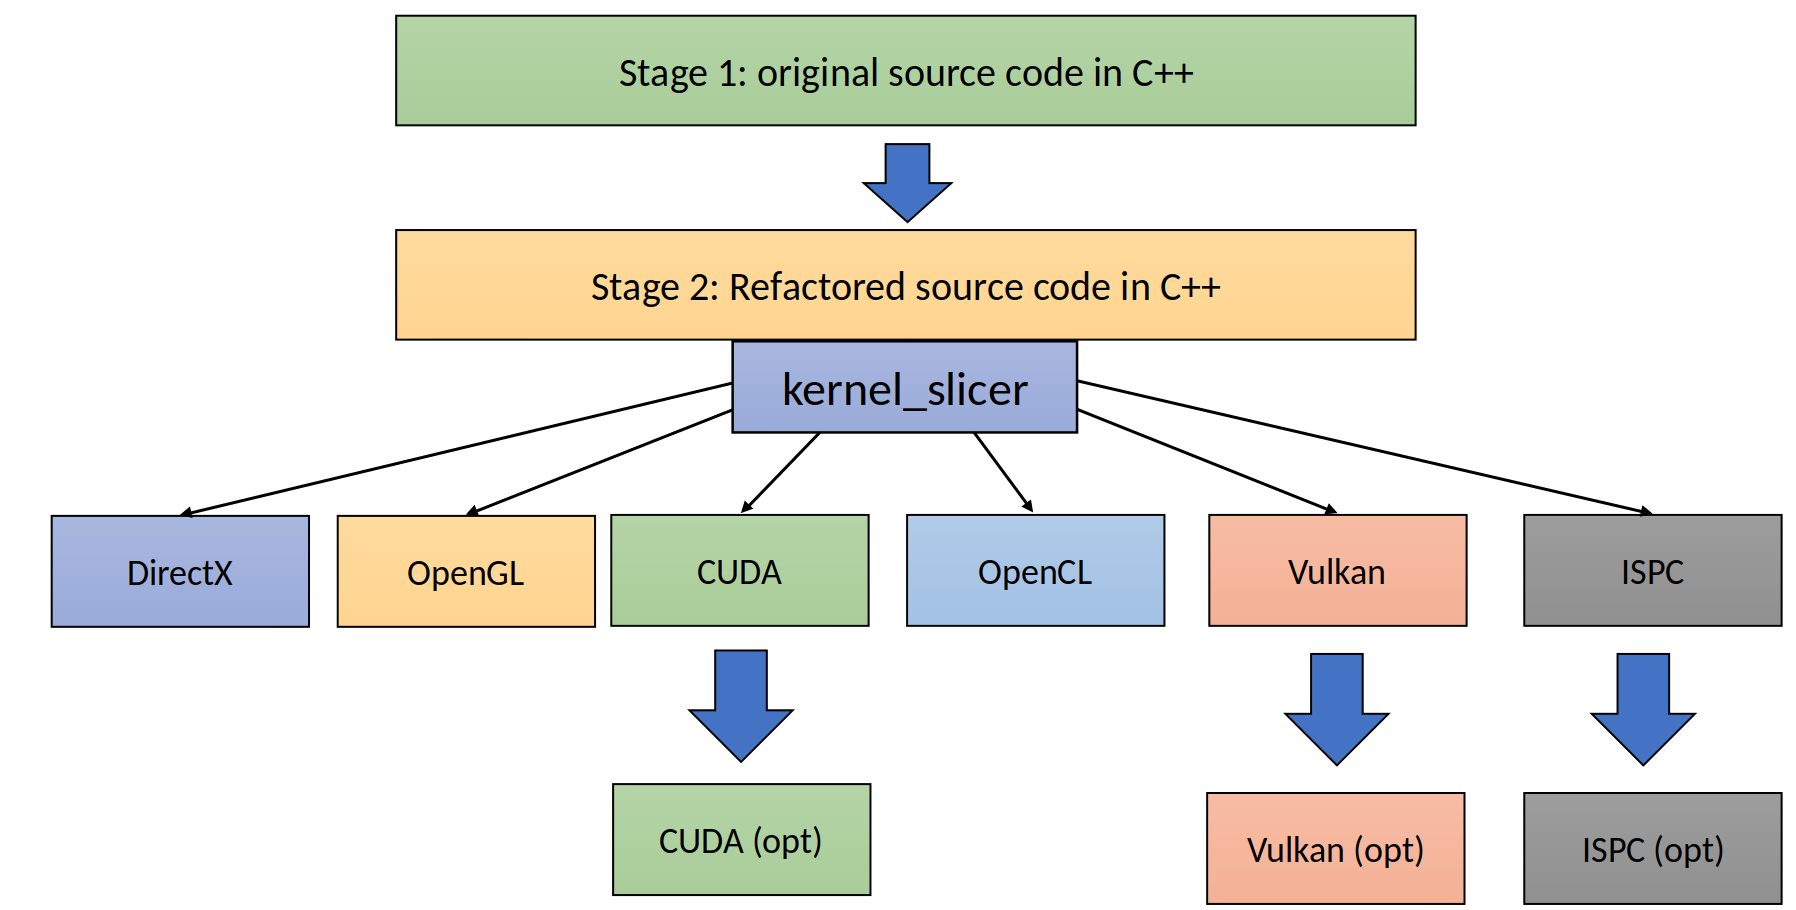
\includegraphics[width=1.0\textwidth]{kslicer_pipeline.jpg}
	\caption{Концепция разработки с kernel\_slicer. На первом этапе Вы разрабатываете свои алгоритмы не задумываясь о GPU вообще. Важно получить работающий код. На втором этапе вы последовательно изменяете С++ код так, чтобы он прошёл через kernel\_slicer. Реализации на различных API/технологиях программирования GPU будут сгенерированы автоматически. На последнем этапе (нижний уровень, CUDA (opt), Vulkan (opt), ISPC (opt)) Вы можете самостоятельно доработать сгенерированный код на каком-то из существующих API через механизм замещения виртуальных функций. При этом если Вам нужны реализации на каких-то других технологиях программирования GPU, который kernel\_slicer не поддерживает в данный момент, Вы всегда можете написать их вручную, сохранив общий интерфейс. }
\end{figure}

\section{Предыстория}\index{Histotry}

Последнее десятилетие технологии программирования GPU (как и других массивно-параллельных вычислительных систем) шли очень непростой дорогой. Эта дорога появилассь в следствии постоянного противоречия между аппаратным ускорением и кросс-платформенностью. 

Когда разработчик полагается на одного производителя вычислительного оборудования (например, Nvidia), вопрос выбора технологии программирования, как правило, остро не стоит. Можно использовать технологии программирования, которые этот производитель поддерживает наилучшим образом \cite{NVCPP,CUDA,OpenACC}. Однако такой подход возможен далеко не всегда. 

Кросс-платформенная разработка (под разные вычислительные системы, центральные процессоры с различными векторными архитектурами, графические процессоры от разных производителей и т.д.)  высоко-производительного ПО представляет собой сложную проблему, для которой в настоящий момент нет простого решения. Основная трудность здесь заключается в том, что аппаратные возможности разных вычислительных систем могут существенно различаться. Поэтому если Вы используете некое аппаратное ускорение на какой-то системе где оно есть, то на системе где оно не поддерживается Вам придётся писать другую версию программы, в которой та же самая функциональность замещяется программно. Как следствие -- либо технология программирования почти не содержит аппаратно-ускоренной функциональности и является почти пустой (как OpenCL), либо получается  Vulkan, который позволяет осуществить доступ к широкому спектру аппаратного ускорения в GPU на большом числе различных устройств. Однако за это приходится расплачиваться повышенной сложностью (рис. \ref{fig:mem}, \ref{fig:vulkan_complexity}). 

\begin{figure}[h]
\begin{minipage}{0.45\textwidth}
	\centering
	
\includegraphics[width=\textwidth]{mem.jpg}
	\caption{Известный мем, пошедший из предложения ``нельзя просто так взять и напасть на Мордор'' в фильме ``Властелин Колец''.}
	\label{fig:mem}
\end{minipage}
\hfill
\begin{minipage}{0.45\textwidth}
	\centering
	
\includegraphics[width=\textwidth]{vulkan_is_hard.png}
	\caption{Простые программы писать на Vulkan сложно, а сложные -- очень сложно.}
	\label{fig:vulkan_complexity}
\end{minipage}
\end{figure}

%\begin{figure}[h]
%	\centering
%	
\includegraphics[width=0.5\textwidth]{mem.jpg}
%	\caption{Известный мем, пошедший из предложения ``нельзя просто так взять и напасть на Мордор'' в фильме ``Властелин Колец''.}
%	\label{fig:mem}
%\end{figure}

К сожалению, работа с этим API как напрямую, так и посредством обёрток/библиотек является довольно трудоёмкой. Например, простейшая отрисовка треугольника может занимать несколько тысяч строк кода. Как следствие растёт стоимость и время разработки. Эта проблема не столько техническая, сколько фундаментальная: она происходит из того, что в Vulkan сочетаются такие противоречивые вещи как кросс-платформенность и аппаратное ускорение. На одних GPU определённое аппаратное ускорение есть, на других его нет,.. на одних оно реализовано таким образом, на других --- по другому. Изначально kernel\_slicer задумывался как инструмент в борьбе со сложностью при работе с Vulkan. Позже он превратился в самостоятельную технологию программирования.

\section{Мотивация Вашей работы с kernel\_slicer }\index{Motivation}

kernel\_slicer не просто позволяет Вам ускорить разработку кода для GPU на Vulkan. Он позволяет делать 4 вещи, которые в других технологиях программирования затруднительно сделать одновременно:

\begin{enumerate}

\item Вы можете сохранить описание своих программ в чистом алгоритимческом виде на обычном С++. Параллельные версии для GPU (Vulkan) и векторных CPU (ISPC) генерируются автоматически. При этом исходная версия может собираться любым существующим компилятором C++. Например, Вы можете также использовать прагмы OpenMP для распараллеливания циклов. Таким образом, kernel\_slicer не делает ваш проект зависимым от себя самого. То есть Вы сегда можете собрать и развивать Вашу программу независимо от того, используете ли Вы kernel\_slicer или нет.

\item Процесс разработки позволяет Вам двигаться мелкими шагами, поэтапно и плавно модифицировать код таким образом, чтобы он в итоге стал параллельным и мог быть перенесён на GPU. Это больше всего похоже на обычный рефакторинг.

\item Вы можете осуществить доступ к любому аппаратному ускорению, доступному в Vulkan и ISPC, даже если текущая версия kernel\_slicer его ещё не поддерживает. Для этого предусмотрен механизм доработки сгенерированного кода. То есть технология рассчитана на это изначально.

\item Если в kernel\_slicer реализована аппаратная поддержка некоторой функциональности, но ваш целевой GPU её не поддерживает, Вы можете заместить неподдерживаемую аппаратную функциональность собственной программной реализацией во время генерации кода.
\end{enumerate}

\begin{remark}Имея опыт работы с различными технологиями (CUDA, OpenCL, DX9-11, OpenGL) и значительную кодовую базу на OpenCL, мы долго не хотели делать свою технологию программирования и рассматривали существующие (Halide, Taichi, HIP и др.). К сожалению, как и в самом OpenCL, всё упиралось в слабую аппаратную поддержку или в жёсткую зависимость от одного производителя. Разработка kernel\_slicer была начата конце 2020-ого года как вынужденная мера по спасению существующих алгоритмических наработок, которые могли потерять актуальность из-за отсутствия аппаратного ускорения. По прошествии 3 лет мы можем сказать, что эта мера сработала. Наши программы более не зависят ни от одного производителя GPU, и вобщем-то, даже от Vulkan они не зависят, т.к. при необходимости мы всегда можем добавить в kernel\_slicer почти любой новый бэк-енд. При этом во время разработки алгоритмической части мы, как правило, вообще забываем про существование GPU.
\end{remark}

%This statement requires citation \cite{book_key}; this one is more specific \cite[122]{article_key}.

%----------------------------------------------------------------------------------------
%	CHAPTER 2
%----------------------------------------------------------------------------------------
\chapterimage{ice_konki1.png}

\chapter{Быстрый старт}

\section{Сборка (Linux)}

\begin{enumerate}
	
\item Склонируйте на свою машину kernel\_slicer и его сабмодули: \begin{itemize}
	\item git clone https://github.com/Ray-Tracing-Systems/kernel\_slicer.git
	\item cd kernel\_slicer
	\item git submodule init
	\item git submodule update
\end{itemize}

\item Установите в своей системе llvm и clang 17-ой версии: \begin{itemize}
	\item wget https://apt.llvm.org/llvm.sh
	\item chmod +x llvm.sh
	\item sudo ./llvm.sh 17
	\item sudo apt-get install llvm-17-dev
	\item sudo touch /usr/lib/llvm-17/bin/yaml-bench
	\item sudo apt-get install libclang-17-dev
	\item sudo apt install clang-17
\end{itemize}

\item Осуществите сборку при помощи CMake: 
\begin{itemize}
	\item cd kernel\_slicer
    \item mkdir cmake-build-release \&\& cd cmake-build-release
    \item cmake -DCMAKE\_BUILD\_TYPE=Release .. 
    \item make -j 8
\end{itemize}

\end{enumerate}

\newpage

\section{Сборка (Windows)}

(*) Для начала скачайте и соберите LLVM-17 по инструкции. \newline https://llvm.org/docs/GettingStarted.html\#getting-the-source-code-and-building-llvm \newline
Используйте следующую конфигуаицию в CMake для LLVM: -DLLVM\_ENABLE\_PROJECTS="clang"
\begin{enumerate}
\item git clone --branch release/17.x --depth=1 https://github.com/llvm/llvm-project.git
\item cd llvm-project
\item cmake -S llvm -B build -G ``Visual Studio 17 2022'' -DLLVM\_ENABLE\_PROJECTS=``clang'' -DCMAKE\_BUILD\_TYPE=Release
\item Откройте файл решения (солюшена) ``llvm-project\\build\\LLVM.sln''и запустите сборку.
\item Сборка время от времени может прерываться с ошибками из-за того что у линковщика заканчивается память. Просто запускайте её снова до тех пор пока все таргеты не будут собраны.
\end{enumerate}

\hspace{3ex}
\newline\noindent (*) Теперь соберите kernel\_slicer используя CMake и VS:
\begin{enumerate}
\item cd kernel\_slicer
\item mkdir cmake-build-release 
\item cd cmake-build-release
\item \begin{verbatim}cmake 
  -DLLVM\_DIR=..\llvm-project\build\lib\cmake\llvm 
  -DClang\_DIR=..\llvm-project\build\lib\cmake\clang 
  -DCMAKE\_BUILD\_TYPE=Release 
  .. \end{verbatim}
\item Откройте файл солюшена \begin{verbatim} ``kernel_slicer\cmake-build-release\kernel_slicer.sln'' \end{verbatim} и запустите сборку.
\end{enumerate}

\section{Сборка в составе LLVM}

Для других операционных систем Вы можете использовать вариант сблоки в составе LLVM.
Инструкция расположена по следующей ссылке:\newline
https://github.com/Ray-Tracing-Systems/kernel\_slicer/blob/master/doc/README\_build\_with\_llvm.md

\pagebreak
\section{Запуск первого примера}

\underline{Шаг 1}: Склонируйте первый туториал из репозитория:

\begin{itemize}
	\item git clone https://github.com/kernel-slicer-tutorials/tutorial1\_vec\_add
	\item cd tutorial1\_vec\_add
	\item git submodule init
	\item git submodule update
\end{itemize}

\vspace*{5px}
Обратите внимание, что туториал, как и сам репозиторий kernel\_slicer использует три существующих репозитория на github: (1) LiteMath для базовых математических операций, (2) vk-utils как легковесную библиотеку хелперов (функций-помошников) для работы с Vulkan и volk (3) для корректной загрузки указателей на функций Vulkan.

\vspace*{5px}
\noindent\underline{Шаг 2}: Соберите программу (пока что на СPU), проанализируйте её исходные коды и убедитесь что она работает: 
\begin{itemize}
	\item mkdir cmake-build-debug \&\& cd cmake-build-debug
	\item cmake -DCMAKE\_BUILD\_TYPE=Debug ..
	\item make -j 2 \textit{// потока только 2  т.к. в CPU версии CMake у Вас мало файлов} 
	\item ./test\_vadd 
\end{itemize}

\vspace*{5px}
\noindent\underline{Шаг 3}: Запустите kernel\_slicer:
\begin{itemize}
	\item Отредактируйте файл run\_kslicer.sh. Измените значение переменной 'kslicer\_directory' так, чтобы она указывала на правильный путь для вашей системы.
	\item bash run\_kslicer.sh 
\end{itemize}

\vspace*{5px}
\noindent\underline{Шаг 4}: Соберите сгенерированный шейдер:
\begin{itemize}
\item cd shaders\_gpu \textit{// будет создана генератором в корне Вашего проекта} 
\item bash build.sh
\end{itemize}

\vspace*{5px}
\noindent\underline{Шаг 5}: Соберите программу (в этот раз уже для GPU) и запустите её:
\begin{itemize}
	\item mkdir cmake-build-debug \&\& cd cmake-build-debug
	\item cmake -DCMAKE\_BUILD\_TYPE=Debug -DUSE\_VULKAN=ON ..
	\item make -j 8 \textit{// здесь файлов будет больше, поэтому потоков 8}
	\item cd ..
	\item ./cmake-build-debug/test\_vadd 
\end{itemize}

Обратите внимание, что запуск производится из основной папки туториала для того чтобы SPIR-V файл корректно загрузился. Вы также можете пользоваться предоставленными конфигами VS Code для сборки, запуска и отладки. Попробуйте зайти внутрь функции 'AddVec' в отладчике.

%\vspace*{5px}
%\noindent\underline{Шаг 6 (опционально)}: Проанализируете сгенерированные файлы.
%\vspace*{2px}
%\noindent Файлы хостового кода:
%\begin{enumerate}
%\item test\_gpu.h -- заголовочный файл для сгенерированного класса
%\item test\_gpu.cpp -- основной код на Vulkan
%\item test\_gpu\_init.cpp -- инициализация Vulkan-объектов
%\item test\_gpu\_ds.cpp -- инициализация дескриптор-сетов
%\item include/Test\_gpu\_ubo.h -- выделенная структура используемых полей класса
%\end{enumerate}

%\vspace*{2px}
%\noindent Файлы шейдеров:
%\begin{enumerate}
%\item shaders\_gpu/build.sh -- последовательность команд для сборки шейдеров	
%\item shaders\_gpu/common\_generated.h -- файл, подключаемый во все шейдеры
%\item shaders\_gpu/kernel1D\_add.comp -- файл шейдера сложения векторов
%\end{enumerate}	

\begin{remark} 
Вы могли заметить, что наш туториал использует кастомный флаг в CMake 'USE\_VULKAN' для опционального подключения Vulkan и задействования GPU версии программы. Если Вы плохо знакомы с CMake, то самое время начать знакомиться с ним. В современном мире разработки ПО это абсолютно необходимо. 
\end{remark}

\chapterimage{ice_fundament.png}
\chapter{Базовые принципы}

Процесс разработки который Вы встретите в туториалах, предполагает, что Вы можете делать несколько различных реализаций ваших алгоритмов на разных технологиях программирования для CPU и GPU. Независимо от того, используете ли Вы kernel\_slicer или нет. 

Кроме того, скорее всего вы захотите реализовывать различные варианты алгоритмов -- более быстрые и простые, либо наоборот, более медленные и качественные. Наконец, входные и выходные данные, как правило, лежат в обычной хостовой памяти (более сложный вариант, когда данные уже в памяти GPU мы рассмотрим в главе \ref{vulkan-direct}). Именно поэтому взаимодействие ваших алгоритмов с внешней средой предполагается реализовывать через простой и очевидный способ --- виртуальные функции с входными и выходными массивами данных. 

\section{Процесс разработки на примере тон-маппинга}\label{tm_example}

Предположим, что Вы хотите написать библиотеку тонирующих операторов (tone mapping). Смысл тон-маппинга довольно прост: на входе у нас есть изображение широкого динамического диапазона (т.н. HDR изображение), которое может содержать произвольные значения яркости в пикселах (float). На выходе у нас т.н. LDR изображение, где все яркости могут быть только целочисленные и в интервале от 0 до 255. Такое изображение уже можно посмотреть на экране монитора. Собственно для этого тонирующие операторы в основном и нужны.

Количество каналов для определённости пусть будет 4. Тогда для каждого пикселя четыре float значения на входе будут превращаться в четыре 8-битных значения на выходе. Это довольно стандартное представление и четыре таких 8-битных значения обычно просто пакуют в один uint32\_t. Делается это, как правило, для того, чтобы при работе с памятью загрузка и сохранение одного пиксела гарантированно превращалась бы в одну инструкцию, загружающую или, соотвественно, сохраняющую понятное количество байт. Не будем нарушать эту традицию (листинг \ref{lst:tonemapping_api2}).

\begin{lstlisting}[language=C++, caption=интерфейс алгоритмов тон-маппинга]
struct IToneMapping
{
  virtual void Run(int width, int height, 
                   const float* in_data,
                   uint32_t* out_data) = 0;
                   
  virtual void Update(...) {}                 
};
\end{lstlisting}\label{lst:tonemapping_api2}

Функция Run будет делать всю работу, но возможно в нашем интерфейсе потребуется объявить дополнительные функции (например Update для задания настроек алгоритма или функции синхронизации, если предполагается, что алгоритм может работать асинхронно с основной программой). Обратите внимание, что входной массив объявлен как const, а выходной не содержит этого спецификатора. Это важно на будущее. Мы считаем in-out массивы плохой практикой с неочевидной семантикой, и kernel\_slicer их не поддерживает (любой не const указатель он воспринимает как out). Если Вы хотите, чтобы один и тот же массив подавался как на вход и на выход, сделайте в вашей функции явно два указателя (один const, другой обычный), и подайте один и тот же указатель как на вход так и на выход явно.  

Но пока что вернёмся к интерфейсу. Мы можем реализовать простой клампинг значений, экспоненциальное отображение или, например, известный алгоритм тон-маппинга Рейнхарда \cite{Reinhard05}. Или что-то более сложное \cite{Mantiuk08}. Для каждой такой реализации Вы скорее всего напишете класс, который будет замещать виртуальную функцию Run. Это является примером нормального и естественного использованием ООП в С++. Очевидно, что в таком случае Вы будете пользоваться этим механизмом и для подключения реализаций на GPU. Давайте считать для определённости, что мы хотим реализовать алгоритм Рейнхарда в классе ReinhardTM (листинг \ref{lst:reinhard}).

\begin{lstlisting}[language=C++, 
	               caption=класс для алгоритма Рейнхарда, 
	               label=lst:reinhard]	
class ReinhardTM : public IToneMapping
{
public:
  void Run(int w, int h, 
           const float* in_data  [[size("w*h*4")]], 
           uint32_t*    out_data [[size("w*h")]]) override;
		   
  void Update(...) override { ... }
   	
protected:
  void kernel1D_findMax(int size, const float*);
  void kernel2D_process(int w, int h, 
                        const float* inpData, 
                        uint32_t*    outData);
  float m_whitePoint;
};
\end{lstlisting}

Далее мы захотим написать классы ReinhardTM\_Vulkan и ReinhardTM\_ISPC, которые будут реализовывать оператор Рейнхарда на GPU и CPU, но уже векторизованным образом, при помощи ISPC. Мы имеем полное право сделать это без участия kernel\_slicer, реализовав соответствующие классы через соответсвующие API программирования GPU самостоятельно. Однако эта работа техническая и достаточно трудоёмкая. Кроме этого, нам придётся повторять её каждый раз, когда CPU версия алгоритма изменится. Для больших программ такая ``поддержка'' может превратиться в настоящий кошмар из-за большого количества деталей, с которыми нам придётся иметь дело при каждом более-менее серьезном обновлении программы. kernel\_slicer позволяет написать только класс ReinhardTM, а параллельные реализации ReinhardTM\_Vulkan и ReinhardTM\_ISPC будут сгенерированы автоматически. Для того чтобы это работало, мы должны следовать нескольким правилам при написании классов.

\section{Основные правила написания класса}

Мы стараемся не добавлять в С++ новых конструкций программирования (за исключением контракта для указания размера массива). kernel\_slicer работает по принципу паттерн-матчинга для того чтобы определить что и как нужно распараллеливать он ищет в вашем коде типичные паттерны. По этой же причине есть некоторые ограничения. Мы дадим список всех паттернов в отдельной главе, а в этом разделе опишем наиболее важные нюансы, которые мы назвали правилами.

\underline{Правило №1:} Всё что внутри Вашего класса -- будет на GPU. Всё что снаружи -- на CPU. Интерфейс вашего класса является естественной границей между CPU и GPU. Думайте о данных вашего класса как об изолированном адресном пространстве.

\underline{Правило №2:} Выполняйте реализацию Ваших алгоритмов изолированно от остальной части программы в одном или нескольких классах. Для каждого такого класса лучше всего делать один или несколько ``.cpp'' файлов. Если в вашем классе есть код, который не должен обрабатываться kernel\_slicer-ом, просто поместите его в отдельный файл. Старайтесь не тянуть в алгоритмическую часть лишние библиотеки из STL и др, если можете обойтись без них.

\underline{Правило №3:} Все ваши алгоритмы должны иметь двух-уровневую организацию. Это функции (т.н. управляющие функции), которые вызывают другие функции (т.н. вычислительные ядра). Код, который должен что-то считать реализуйте внутри функций-ядер. Код, который управляет запуском ядер (например в зависимости от значения параметра запускает один или другой кернел) реализуйте в управляющих функциях (листинг \ref{lst:RunFunc}). Код вычислительных ядер выполняется на GPU, код управляющих функций --- на CPU.

\begin{lstlisting}[language=C++, 
	               caption=реализация управляющей функции вызывающей вычислительные ядра, 
	               label=lst:RunFunc]	
void ReinhardTM::Run(int width, int height, 
                     const float* in_data, 
                     uint32_t* outData)
{
  kernel1D_finMax(in_data, width*height);
  kernel2D_process(width,height,in_data,outData);
}
\end{lstlisting}

\underline{Правило №4:} Вычислительные ядра должны содержать в имени префикс kernel1D\_, kernel2D\_ или kernel3D\_. Число перед буквой D указывает на то, сколько вложенных циклов нужно параллелить. Остальные циклы и все функции вызываемые из них будут вставлены в код шейдера (листинг \ref{lst:kernel2D_process}). 

\underline{Правило №5:} Массивы/указатели в аргументах управляющих функций могут быть либо ``строго in'' (const float*), либо ``строго out (float*)''. Семантика inout не разрешена (для не констнатных указателей не будет сгенерирован код копирования данных на gpu, только обратно код копирования с gpu на cpu). При этом для всех массивов/указателей необходмо в двойных квадратных скобках указать их размер, как выражение зависящее от аргументов управляющей функции.  

\begin{remark}
Конструкция [[size("N")]] нужна для того чтобы сгенерировать корректный код копирования данных на GPU и обратно. Она не является директивой параллельного программирования. Вы можете относиться к этой конструкции как к контракту. Разработчик класса обещает пользователю этого класса, что он считает не более чем N элементов массива для входных аргументов или что он запишет не более чем N элементов массива для выходных аргументов. 
\end{remark}	

\underline{Правило №6:} Количество итераций для параллельных циклов должно: либо (1) передаваться через аргументы функций-ядер, либо (2) быть переменной, являющейся членом класса. Если Вам нужно вычислить это количество каким-то образом, Вы можете сделать это двумя путями.
\begin{enumerate}
\item Вычислить это число в управляюшей функции, как в нашем примере, где вычисляется произведение width*height для ядра kernel1D\_findMax. В этом случае эти вычисления будут произведены на CPU.
\item Вычислить это число в другом вычислительном ядре и сохранить его в переменной, являющейся членом класса. Такая переменная должна непосредственно учавствовать далее в выражении for в качестве количества итераций цикла в тех ядрах, которые предполагается запускать этим способом. Забегая вперёд скажем, что это т.н. непрямой вызов вычислительного ядра (indirect dispatch), когда количество итераций/микро-потоков станет известно лишь в момент выполнения программы на GPU. 
\end{enumerate}

\begin{lstlisting}[language=C++, 
	               caption=двумерное вычислительное ядро вызывает функцию reinhard\_ext, 
	               label=lst:kernel2D_process]	
float reinhard_ext(float v, float max_white)
{
  float numerator = v * (1.0f + (v / (max_white * max_white)));
  return numerator / (1.0f + v);
}

void ReinhardTM::kernel2D_process(int width, int height, 
                                  const float* in_data, 
                                  uint32_t* outData)
{
  for(int y=0;y<height;y++) // first par. loop (kernel2D_)
  {
    for(int x=0;x<width;x++) // second par. loop (kernel2D_)
    {
      float r = reinhard_ext(in_data[4*(y*width+x)+0], m_whitePoint);
      float g = reinhard_ext(in_data[4*(y*width+x)+1], m_whitePoint);
      float b = reinhard_ext(in_data[4*(y*width+x)+2], m_whitePoint);
			
      int ir  = (int)std::min(r*255.0f, 255.0f);
      int ig  = (int)std::min(g*255.0f, 255.0f);
      int ib  = (int)std::min(b*255.0f, 255.0f);
			
      outData[y*w+x] = 0xFF000000 | (ib << 16) | (ig << 8) | ir;
    }
  }
}
\end{lstlisting}


\underline{Правило №7:} Вы можете передавать данные из управляющей функцией в ядро только через аргументы ядра. Нельзя, например, записать значение переменной члена класса в управляющей функции и прочитать его в ядре: на GPU прочитается старое значение.

\underline{Правило №8:} Вы можете передавать данные между различными вычислительными ядрами либо (1) через их аргументы (как в нашем примере, где оба вычислительных ядра принимают на вход один и тот же указатель in\_data), либо (2) через члены класса. Члены класса могут иметь типы данных std::vector<...> и LiteImage::Image2D<...>. Для Вулкана каждый vector превратится в VkBuffer, a Image2D в VkImage.

\underline{Правило №9:} В качестве членов класса и в любых буферах (std::vector<...>) cтарайтесь использовать типы данных, размер которых кратен 4 (int/float), 8(int2/float2) или 16 байтам (int4/float4). 

\begin{remark}
Это правило не связано с самим kernel\_slicer-ом, оно связано с правилами выравнивания структур данных в GLSL, которые довольно мутные. В кратце, если в вашей структуре встречается выровненный по 8-байтной границе тип данных (например float2 или double), размер самой структуры должен быть кратен 8 байтам. А если в структуре встречается тип выроненный по 16-байтовой или более границе (float4), то нужно выравнивать на 16 байт. Лучше всего в этом случае, явно добавить неиспользуемые члены данных в вашу структуру.
\end{remark}

\begin{remark}
Тип данных float3/vec3 весьма коварен. Его размер на CPU обычно 12 байт. Однако его размер на GPU зависит от того, как он используется. Если он является членом структуры, в которой есть, например, ещё один float, тогда vec3 будет занимать 12 байт, а сама структура --- 16 байт. Однако если обратиться по индексу к буферу, в котором хранятся vec3, то сам тип данных vec3 будет уже занимать 16 байт. Такое поведение невозможно корректно реализовать на CPU, поэтому мы не рекомендуем Вам хранить что-то во float3. При этом в рассчётах его можно свободно использовать. То есть в качестве локальныйх переменных или аргументов функций.
\end{remark}	

\underline{Правило №10:} Понимайте ограничения графических процессоров. На GPU многие вещи делать не позволяется. Нельзя делать рекурсию (её нужно преобрабовывать в алгоритм, который явно работает со стэком). Нельзя динамически выделять память, а следовательно, создавать новые вектора или умные указатели в коде вычислительных ядер. В технологии программирования мы не можем и не должны обходить аппаратные ограничения. Наоборот, лучше всего сделать так, чтобы неэффективный код было трудно или невозможно написать.

\chapterimage{baikal2.jpg}
\section{Измеряем время выполнения и копирования}

Ранее мы опустили некоторые детали. Например, Вы могли заметить, что в тестовом классе присутствуют функции CommitDeviceData и GetExecutionTime, которые никак не использовались. Посмотрим для чего они нужны на примере того же алгоритма тон-маппинга.

\noindent\underline{Шаг 1}: Склонируйте второй туториал из репозитория:

\begin{itemize}
	\item git clone https://github.com/kernel-slicer-tutorials/tutorial2\_reinhard\_tm
	\item cd tutorial2\_reinhard\_tm
	\item git submodule init
	\item git submodule update
\end{itemize}

\vspace*{5px}
\noindent\underline{Шаги 2--5}: повторите шаги 2--5 из главы быстрый старт для этого туториала. 

\vspace*{5px}
\noindent\underline{Шаг 6}: Обратите внимание на механизм измерения времени при помощи функции GetExecutionTime. 

В своём классе Вы самостоятельно реализуете оценку времени работы каждой управляющей функции (например ``Run'') на CPU и сохранение её времени работы в какой-либо внутренней переменной. GetExecutionTime позволяет получить это время по имени функции, переданной ей через аргумент. Поскольку в нашем примере в классе только одна управляющая функция (Run), мы можем игнорировать имя функции и всегда записывать в выходной аргумент время выполнения функции Run. В общем случаем нам придётся доработать этот код, чтобы для разных входных имён функций в GetExecutionTime мы получали корректное значение времени выполнения. В сгенерированном классе kernel\_slicer будет замещать эту функцию собственной реализацией. Результат Вы получаете в выходном массиве в виде 4 значений: 

\begin{enumerate}
\item время выполнения на GPU;
\item время копирования входных данных с CPU на GPU;
\item время копирования выходных данных с GPU на CPU;
\item время, затраченное на накладные расходы в API программирования GPU.
\end{enumerate}

\section{Алгоритмический паттерн-матчинг в kernel\_slicer}

Тон-маппинг Рейнхарда не такой простой, каким кажется на первый взгляд. В его расширенной версии на первом этапе требуется найти максимальный уровень яркости по всему изображению. Казалось бы, в чём проблема? Ведь поиск максимума --- это тривиальная задача (листинг \ref{lst:kernel1D_finMax}).

\begin{lstlisting}[language=C++, 
  	               caption=вычислительное ядро поиска максимума с алгоритмическим паттерном редукции, 
	               label=lst:kernel1D_finMax]	
void ReinhardTM::kernel1D_finMax(const float* hdrData, int size)
{
  m_whitePoint = 0.0;
  for(int i=0;i<size;i++)
  {
    float r = hdrData[4*i+0];
    float g = hdrData[4*i+1];
    float b = hdrData[4*i+2];
    float maxValue = std::max(r, std::max(g,b));
    m_whitePoint = std::max(m_whitePoint, maxValue);
  }  
}
\end{lstlisting}

К сожалению это не так. Дело в том, что параллельный поиск максимума на GPU можно реализовать эффективно только через параллельную редукцию -- алгоритм, который довольно трудоёмко реализовывается и, кроме того, имеет ряд нюансов в зависимости от GPU и типа данных (float/int), над которым производится редукция. 

А именно, для целочисленных операций существуют атомарные операции, которые можно использовать уже после локальной редукции в рабочей группе потоков. А вот для плавающей точки аппаратной поддержки как в Vulkan, так и в других технологиях программирования просто нет. Следовательно, после редукции в рабочей группе Вам придётся сохранить промежуточные данные в какой-то отдельный буфер и запустить операцию редукции ещё раз. А значит нужно выделять память, создавать отдельные ресурсы и запускать отдельные вычислительные ядра. Наконец, саму редукцию внутри рабочей группы можно делать немного по-разному.

kernel\_slicer обнаруживает редукцию в вашем коде, ориентируясь на паттерн доступа к переменной внутри цикла, являющейся членом класса. Далее он генерирует весь необходимый код в зависимости от типа переменной и входных настроек (например, с использованием subgroups или без них), см. листинг \ref{lst:finMaxShaders}.

\begin{lstlisting}[language=C++, 
	               caption=Фрагмент сгенерированного GLSL шейдера для параллельной редукции, 
	               label=lst:finMaxShaders]	

shared float m_whitePointS[256*1*1]; 

void main()
{	               
  const uint lid = gl_LocalInvocationID[0];
  ...	               
  float r = hdrData[4*i+0];
  float g = hdrData[4*i+1];
  float b = hdrData[4*i+2];
  float maxValue = max(r, max(g, b));
  m_whitePointS[lid] = max(m_whitePointS[lid], maxValue);
  ...
  barrier();
  if (lid < 128) 
  	m_whitePointS[lid] = max(m_whitePointS[lid],m_whitePointS[lid+128]);
  barrier();
  if (lid < 64) 
  	m_whitePointS[lid] = max(m_whitePointS[lid],m_whitePointS[lid+64]);
  barrier();
  if (lid < 32) 
  	m_whitePointS[lid] = max(m_whitePointS[lid],m_whitePointS[lid+32]);
  ...
}  
\end{lstlisting}

Таким образом, Вы можете сохранить описание вашего алгоритма в простом виде с последовательной логикой, и не заниматься самостоятельной реализаций по крайней мере для некоторых часто-используемых примитивов параллельного программирования. В главе \ref{patterns} Вы найдёте описание всех реализованных алгоритмических паттернов.

\begin{remark}
Посмотрите как делается параллельная редукция в OpenMP. В kernel\_slicer мы не стали добавлять специальные директивы для указания перменных для которых следует генерировать параллельную редукцию. Мотивация которой мы руководствовались заключается в том, что подобный паттерн является слишком очевидным, и его проще запомнить в алгоритмическом виде, чем в виде отдельной директивы или конструкции языка. Попробуйте воспроизвести по памяти пример параллельной редукции из OpenMP. 
\end{remark}

\chapterimage{ice_problems.jpg}
\chapter{Частые проблемы и пути их решения}

\section{Проблемы подключаемых библиотек и файлов}

\subsection{\underline{Проблема №1}: Не найден подключаемый файл либо \underline{странные конфликты} определений типов в библиотечных файлах gcc}

Например, это может звучать так: kernel\_slicer пытается найти stddef.h не в TINYSTL, а в стандартной библиотеке GCC 11. 

С этой проблемой Вы скорее всего рано или поздно столкнётесь. Попробуйте, например подключить  файл <functional> или <bitset>. Сообщение об ошибке может зависеть от операционной системы в которой Вы работаете, поскольку это немного зависит от поведения clang-а. Если повезёт, то Вы получите недвусмылсенное сообщение о том, что файл <functional> не найден. Однако чаще можно встретить следующее:

\begin{lstlisting}[language=C++, 
	caption=ошибка из-за ненайденного файла bitset из STL, 
	label=lst:filenotfound]	
/usr/lib/gcc/x86_64-linux-gnu/11/../../../../include/x86_64-linux-gnu/c++/11/bits/c++config.h:281:28: error: typedef redefinition with different types ('long' vs 'unsigned long')
typedef __PTRDIFF_TYPE__      ptrdiff_t;
                                 ^
kernel_slicer/TINYSTL/cstddef:10:25: note: previous definition is here
  typedef unsigned long ptrdiff_t;
                        ^
In file included from ... :
In file included from /usr/lib/gcc/x86_64-linux-gnu/11/../../../../include/c++/11/bitset:50:
In file included from /usr/lib/gcc/x86_64-linux-gnu/11/../../../../include/c++/11/iosfwd:39:
/usr/lib/gcc/x86_64-linux-gnu/11/../../../../include/c++/11/bits/stringfwd.h:79:33: error: typedef redefinition with different types ('basic_string<char>' vs 'str::string_base<char>')
\end{lstlisting}

\noindent\underline{Причина}: clang не находит файл в списке своих ``include directories'', после чего он начинает лезть с операционную систему и искать инклюды там. Находит инклюды от gcc, что ему в принципе противопоказано, и ломается. 

\vspace*{5px}
\noindent\underline{Решение 1.1}: Лучше всего выделить код, которому нужны специфические библиотеки в отдельные файлы, которые вообще не будут обрабатываться слайсером. А код, который должен обрабатываться поместить в файлы, не тянущие за собой лишних библиотек. Кроме всего прочего это улучшает архитектуру программы т.к. позволяет отделить алгоритмы от вспомогательной или системной функциональности.

\vspace*{5px}
\noindent\underline{Решение 1.2}: Добавьте путь к библиотеке в список ``include directories'' для того чтобы транслятор смог найти нужные файлы. Обычно эта рекомендация относится к вашим собственным или другим нестандартным (то есть не-STL) библиотекам. Делается это через аргументы командной строки следующим образом (листинг \ref{lst:addincludes}):

\begin{lstlisting}[caption=добавляем новый подключаемый файл, 
	label=lst:addincludes]	
-IMy/Path/To/Library1 "ignore"
-IMy/Path/To/Library2 "process"
\end{lstlisting}

Используйте вариант с ``ignore'' по умолчанию. Так Вы сообщаете слайсеру, что не хотите чтобы код из этих директорий обрабатывался им и переносился в шейдер -- достаточно их просто подключить чтобы корректно распарсить С++. Если же Вам нужно переносить код из каких-то подключаемый файлов на GPU (как правило это только Ваши собственный библиотеки), поместите их в отдельную директорию и используйте второй вариант с ``process''.

\begin{remark}
Папка ``include'' в директории, где находится первый из обрабатываемых слайсером файлов (если их несколько) всегда рассматривается слайсером с опцией ``process''.
\end{remark}

\vspace*{5px}
\noindent\underline{Решение 1.3}: Просто добавьте в kernel\_slicer/TINYSTL нужный файлы или определения функций и типов данных. Реализовывать их \underline{не нужно(!!!)}, достаточно только определить, чтобы clang распарсил C++. Это решение относится к ситуации, когда Вы всё-таки хотите смешивать в одном файле алгоритмы и некоторую библиотечную функциональность из STL, которая не определена в данный момент в TINYSTL. Вы можете сделать пулл-реквест или просто направить исправленные версии TINYSTL нам.

\vspace*{5px}
\noindent\underline{Решение 1.4}: (Если не найдены базовые вещи которые точно должны работать, например vector). На ArchLinux и Windows мы сталкивались со специфическим поведением clang. Он ищет какие-то свои специальные библиотеки в папке ``../lib/clang/17.0.0/include'' относительно той папки, из которой он запускается. Нужно создать такую папку и скопировать туда содержимое из ``llvm17/build/lib/clang/17.0.0/include'', которая есть в llvm соответсвующей версии (можете скачать у них с github). История это проблемы здесь: https://github.com/Ray-Tracing-Systems/kernel\_slicer/issues/4

\subsection{\underline{Проблема №2}: В STL не наден какой-то определённый тип данных или функция.}

\noindent\underline{Причина}: мы используем свою версию библиотеки STL на базе существующей библиотеки TINYSTL. Нюанс в том, что слайсеру не нужна реализация STL, достаточно только иметь корректные определения интерфейсов. По некоторым причинам нам действительно удобнее иметь свою версию STL. Смотрите решение 1.3 предыдущей проблемы.

\section{Проблемы обработки исходного кода}

\subsection{\underline{Проблема №3}: Потерянная функция или тип данных.} kernel\_slicer говорит, что функция не найдена, хотя она у Вас точно есть. Либо функция не переносится в шейдер, хотя по логике вроде должна т.к. шейдер из-за этого не собирается.

\noindent\underline{Причина}: Скорее всего kernel\_slicer просто не видит файл, в котором объявлена эта функция. \underline{Решение}: Проверьте аргументы командной строки, с которыми Вы запускаете слайсер. Убедитесь, что файл, в котором определена ваша функция либо явно передаётся в слайсер, либо подключается в одном из передаваемых явно файлов. Слайсер умеет обрабатывать несколько файлов. Просто передавайте их как 1, 2, 3 и т.п. аргументы командной строки разделённые проблелом.  

\subsection{\underline{Проблема №4}: Некоторые строчки кода в шейдерах съедены/испорчены, либо наоборот добавляется мусор в конце строки.}

\noindent\underline{Причина}: Мы полагаем, что эта проблема вызывана багом в т.н. front-end части самого clang. Она происходит из-за двойного преобразования текста (т.н. rewrite) в некоторых узлах AST дерева, связанных с неявными преобразованиями типов данных. 

\vspace*{5px}
\noindent\underline{Решение №4.1}: Разбейте в вашем исходном коде такие строчки на несколько более простых строк, чтобы уменьшить число выполняемых преобразований текста на одну строку. Заодно и читаемость кода улучшится.

\vspace*{5px}
\noindent\underline{Решение №4.2}: Сделайте все или хотя бы некоторые преобразования типов данных в ваших выражениях явными. 

\subsection{\underline{Проблема №5:} В шейдеры переносится код, который не нужно туда переносить.}

\noindent\underline{Причина}: Алгоритм, который определяет зависимости в коде не совершенен. \underline{Решение}: Используйте макросы условной компиляции вида \#ifndef KERNEL\_SLICER чтобы убрать из обработки определённый код. Либо вынесите этот код в отдельный файл.  

%\section{Другие известные проблемы}
%\underline{Проблема:} Макрос MAXFLOAT пропадает. \underline{Решение:} Подключите файл <cfloat> и используйте FLT\_MAX.

\chapterimage{ice_patterns.jpg}
\chapter{Паттерны}\label{patterns}

\section{Паттерны в вычислительных ядрах}

\noindent\underline{Редукция}.

\begin{lstlisting}[language=C++, 
	               caption=паттерн редукции, 
	               label=lst:reduction]		
void Numbers::kernel1D_ArraySumm(const int* a_data, size_t a_dataSize)
{
  m_summ = 0; 
  for(int i=0; i<a_dataSize; i++) {
    if(a_data[i] > 0)
      m_summ += a_data[i];
    //the general form is m_summ = f(m_summ, ...); 
  }
}
\end{lstlisting}

Где m\_summ -- переменная, являющаяся членом класса.

\noindent\underline{Добавление элементов в буфер}.

Вы можете вызывать внутри выяислительных ядер функцию ветора push\_back(...), чтобы складывать элементы в его конец (листинг \ref{lst:redpixels}). Однако здесь есть два важных нюанса:

\begin{enumerate}
\item Добавление элементов в буфер будет реализовано через атомарный счётчик. Такой алгоритм не сохраняет исходный порядок, в котором элементы добавляются в вектор. Если Вам нужно сохранить порядок -- сначала запишите их самих или их индексы в отдельный буфер, а затем используйте префиксную сумму в управляющей функции (подробнее об это см. про префиксные суммы).
\item На GPU вектор может изменить свой size(), но не может изменить capacity(). Следовательно, перед тем как добавлять элементы в вектор, Вам нужно зарезервировать его на CPU (до вызова функции CommitDeviceData) на достаточный для вашей задачи размер. Не поместившиеся в capacity() элементы не будут добавляться в вектор.
\end{enumerate}

\begin{lstlisting}[language=C++, 
	               caption=добавление элементов в конец буфера, 
	               label=lst:redpixels]	
void RedPixels::kernel1D_FindRedPixels(const uint32_t* a_data, 
                                       size_t a_dataSize)
{
  m_foundPixels.resize(0);
  for(uint32_t i = 0; i<a_dataSize; i++) {
    const uint32_t pixValue = a_data[i];
    if(PixelIsRed(pixValue)) {
      PixelInfo info;
      info.index = i;
      info.value = pixValue;
      m_foundPixels.push_back(info);
    }
  }
}
\end{lstlisting}

\noindent\underline{Непрямой вызов ядра}.

Как уже ранее упоминалось, Вы можете записать значение некоторой переменной в одном кернеле (ядре), а затем использовать эту переменную в качестве выражения для указания количества итераций цикла в другом кернеле (ядре). Можно использовать также функцию size() у вектора (листинг \ref{lst:indirect_dispatch}). Это особенно полезно в сочетании с предыдущим паттерном или с префиксной суммой. Вы можете сначала плотно сложить в буфер ровно столько элементов сколько нужно, а затем вызвать новое вычислительное ядро только для добавленных ранее элементов.

\begin{lstlisting}[language=C++, 
	               caption=непрямой вызов ядра, 
	               label=lst:indirect_dispatch]	
void RedPixels::kernel1D_IndirectDispatchExample(uint32_t* a_data)
{
  for(uint32_t pixelId = 0; pixelId < m_foundPixels.size(); pixelId++) {
  	...
  }
}
\end{lstlisting}

Поскольку до момента выполнения предыдущего ядра размер вектора m\_foundPixels просто неизвестен.

\noindent\underline{Обращение к текстурам}.

Для работы с текстурами используйте тип данных LiteImage::Image2D<...>. Здесь следует различать запись, чтение и сэмплирование.

\noindent\underline{Массивы текстур}.

Для работы с массивом текстур используйте интерфейс ICombinedImageSampler.
Указатели на этот тип данных нужно сложить в std::vector. Поскольку текстуры могут быть разного размера, из таких массиво можно только сэмплировать данные.

\begin{lstlisting}[language=C++, 
	caption=сэмплирование из массива текстур, 
	label=lst:texarrays]	
class TestCombinedImage {
  ...  
  std::vector< std::shared_ptr<ICombinedImageSampler> > m_textures;
  std::vector< const ICombinedImageSampler* >           m_textures2;
};

void TestCombinedImage::kernel2D_Run(const int a_width, const int a_height, 
                                     unsigned int* outData1ui)
{
  for (int y = 0; y < a_height; ++y) {
    for (int x = 0; x < a_width; ++x) {  
      ...
      int dynamicId = ... ;			
      float4 color  = m_textures[dynamicId]->sample(uv); 
      float4 color2 = m_textures2[dynamicId]->sample(uv);     
      ...
    }
  }
}
\end{lstlisting}

В Vulkan такие массивы --- это отдельная функциональность, называемая \newline ``VK\_EXT\_descriptor\_indexing''. 

\noindent\underline{Пересечение луча и поверхности (т.н. Ray Query)}.

Используйте интерфейс ISceneObject из библиотеки LiteRT/CrossRT \cite{litert} для того чтобы задействовать в сгенерированном коде аппаратное ускорение трассировки лучей.

\begin{lstlisting}[language=C++, 
	caption=поиск пересечения луча и поверхности, 
	label=lst:ray_query_hit]

  const float4 rayPosAndNear = ...;
  const float4 rayDirAndFar = ... ;		
  CRT_Hit hit = m_pAccelStruct->RayQuery_NearestHit(rayPosAndNear, 
                                                    rayDirAndFar);

\end{lstlisting}

\begin{remark}
Не следует путать паттерн Ray Query с паттерном трассировки лучей о котором пойдёт речь в следующем разделе. 
\end{remark}

\noindent\underline{Указатель + смещение в аргументах функций}.

Поскольку в GLSL нет указателей, а в С++ они есть, далеко не любой код легко преобразовать из С++ в GLSL. Однако поскольку в С++ использование указателей и передача их в аргументы функций является супер-частым приёмом, нам пришлось реализовать поддержку указателей в некотором ограниченном виде (листинг \ref{lst:addptr}). 

Если Вы знакомы с OpenCL, то знаете что в нём указатели разделяются на локальные (которые просто указывают на какие-то локальные переменные кернела) и глобальные, которые указывают на настоящую память. В OpenCL Вы должны явно указывать для всех указателей, какого типа они будут т.к. заранее непонятно, что именно за указатель пришёл к Вам в функцию. 

В kernel\_slicer этого делать не нужно, т.к. мы не допускаем произвольную арифметику указателей. Но фактическое разделение на глобальные и локальные указатели есть.

\begin{itemize}
\item Локальный указатель  --- это указатель на локальную переменную ядра.  
\item Глобальный указатель -- это указатель, передаваемый в ядро через аргумент, либо указатель на начало некоторого вектора (m\_materials.data() в листинге \ref{lst:addptr}). Для них требуется дополнительная работа.
\end{itemize}

\noindentИтак, у Вас есть следущие возможности:

\begin{enumerate}
\item И локальные, и глобальные указатели Вы можете передавать в аргументы функций. 
\begin{itemize}
\item В текущей версии поддерживается только 1 уровень вложенности для глобальных указателей. Но мы \href{https://github.com/Ray-Tracing-Systems/kernel_slicer/issues/16}{обещаем это исправить} \cite{issue16}.
\item Локальные указатели при трансформации в GLSL, как и ссылки, просто превращаются в inout аргументы.
\end{itemize}	
\item Для глобальных указателей Вы можете использовать арифметику указателей, но только на сложение, и только в аргументах вызывамых функций (листинг \ref{lst:addptr}).
\item Внутри функции, куда Вы передаёте глобальный указатель, обращайтесь к указателю как к массиву. Даже если там только 1 элемент, используйте выражение ``data[0]'' чтобы его прочитать. 
\end{enumerate}

\begin{lstlisting}[language=C++, 
	caption=ограниченная поддержка арифметики указателей, 
	label=lst:addptr]
  myfunc(m_materials.data() + currMatId, ...);
\end{lstlisting}

\section{Паттерны в управляющих функциях}

\noindent\underline{Префиксная сумма}. Вы можете использовать std::exclusive\_scan и std::inclusive\_scan в управляющих функциях.

\noindent\underline{Сортировка}. Вы можете использовать std::sort с лямбда-выражением (это обязательно) в управляющих функциях. Будьте внимательны: размер сортируемого массива в данный момент должен быть кратен степеням двойки т.к. слайсер втавляет алгоритм битонической сортировки, имеющий такое ограничение.

\noindent\underline{Трассировка лучей (архитектурный паттерн)}.

Особенность приложений трассировки лучей в том, что в них, как правило, нет какого-то неравномерного изменения количества потоков или сложных параллельных алгоритмов. Все лучи работают абсолютно параллельно и одинаково.

Однако сам код на 1 луч может довольно сложным. Далее про убер-ядра и раздельные ядра ... **UNDER CONSTRUCTION** ...  

\begin{remark}
Большинство паттернов можно разделить по тому, где они должны встречаться: в вычислительных ядрах или в управляющих функциях. Однако некоторые паттерны могут встречаться и там и там. В качестве примере можно привести доступ к основным членам класса std::vector: begin(), end(), size(), capacity().
\end{remark}

\chapterimage{nerpa_functions.jpg}
\chapter{Специальные функции}\label{spec_functions}

kernel\_slicer предполагает, что в вашем классе могут быть реализованы некоторые специальные функции. Если такие есть, он их замещает, если нет -- генерирует при необходимости. В исходном классе, как правило, такие функции будут пустыми, поскольку они не имеют смысла для CPU реализации. Исключение составляет функция GetExecutionTime, которую Вы можете реализовать самостоятельно, если хотите измерять время выполнения алгоритма на CPU.

\begin{enumerate}
	\item Name() --- возвращает имя текущего класса. 
	
	\item GetExecutionTime(...) --- получение статистики по времени выполнения (и копирования данных) для определённой управляющей функции по её имени.
	\item CommitDeviceData(...) --- копирование данных класса на GPU (CPU => GPU). Копируются только те данные, доступ к которым осуществляется из вычислительных ядер. 
	
	\item UpdateMembersPlainData(...) --- обновление (CPU => GPU) только тех членов класса, которые являются т.н. Plain Old Data (POD) и для которых встречается обращение на GPU. Обраните внимание, что в отличие от предыдущей функции эта функция не копирует вектора и текстуры и является достаточно легковесной.
	
	\item ReadPlainMembers(...) --- чтение (CPU <= GPU) POD данных класса обратно в память на CPU. Эта функция вызывается в конце работы каждой сгенерированной управляющей функции и забирает новое состояние класса наряду с дургими данными которые необходимо копировать с GPU обратно в т.н. хост-память CPU.
	
	\item UpdateMembersVectorData(...) --- обновление всех векторов (CPU => GPU).
	
    \item UpdateMembersTextureData(...) --- обновление всех текстур (CPU => GPU).
    
    \item ListRequiredDeviceFeatures(...) --- статическая функция, позволяющая получить список аппаратных функциональностей, необходимых для сгенерированного класса. Эта функция не замещается слайсером.
    
    \item InitVulkanObjects(...) --- функция инициализации всех ресурсов Vulkan для данного класса. Должна быть вызвана сразу после конструктора сгенерированного класса. Она может понанобится Вам в главе \ref{vulkan-direct}. Эта функция не замещается слайсером.
    
    \item SceneRestrictions(...) --- функция для задания ограничений на сцену. Нужна для того чтобы корректно проинициализировать структуры данных Вулкана, связанные с аппаратным ускорением трассировки лучей. Эта функция на выходе даёт 4 значения в массиве (листинг \ref{lst:SceneRestrictions}). Она вызывается из функции InitVulkanObjects() сразу после работы конструктора сгенерированного класса, поэтому для корректной работы Вам, возможно придётся передавать в неё некоторые данные через статические функции и члены Вашего исходного класса. Эта функция не замещается слайсером. Вы должны реализовать её самостоятельно если хотите делать трассировку лучей для больших сцен. Насколько больших -- как раз она и определяет.
     
\end{enumerate}

\begin{lstlisting}[language=C++, 
	               caption=Пример реализации функции SceneRestrictions, 
	               label=lst:SceneRestrictions]	 
virtual void SceneRestrictions(uint32_t a_restrictions[4]) const
{
  uint32_t maxMeshes            = 1024;
  uint32_t maxTotalVertices     = 1000000;
  uint32_t maxTotalPrimitives   = 1000000;
  uint32_t maxPrimitivesPerMesh = 200000;
	
  a_restrictions[0] = maxMeshes;
  a_restrictions[1] = maxTotalVertices;
  a_restrictions[2] = maxTotalPrimitives;
  a_restrictions[3] = maxPrimitivesPerMesh;
}               
\end{lstlisting}

\chapterimage{ice_cmd.jpg} % Chapter heading image
\chapter{Параметры командной строки}

\begin{enumerate}
\item -mainClass "MyClass" \thinspace---\thinspace имя класса, который будет подвергаться обработке;
\item -stdlibfolder --- "Path/To/TINYSTL" путь к нашей версии STL;

\item -shaderCC ``glsl''. Задаёт тип бэк-енда. В данный момент позволяет выбирать между тремя вариантами: (1) Vulkan + шейдеры GLSL (``glsl''), (2) Vulkan + шейдеры в OpenCL через clspv ``opencl'' (deprecated), (3) реализация на ISPC (``ispc''); 

\item -shaderFolderPrefix "My/Path/To/Shaders". Позволяет задать путь к шейдерам. 

\item -suffix ``\_GPU''. Суффикс, который будет дописан к имени сгенерированного класса и папки с шейдерами.

\item -reorderLoops "YX". Позволяет переупорядочить циклы. Обычно это нужно для алгоритмов обработки изображений, осуществляющих доступ к двумерным данным. В CPU коде, как правило, во внешнем цикле итерируют по Y, а во внутреннем -- по X. Это делается для того при ``pitch-linear'' расположении данных/пикселей в буфере не происходил  разрыв адреса во внутреннем цикле;

\item -pattern ``ipv'' --- задаёт глобальное поведение слайсера при обработки класса. Значение ``ipv'' расшифровывается как Image Processing Vectorization, и означает обычный тип управляющих функций. Значение ``rtv'' расшифровывается как Ray Tracing Vectorization и используется для приложений трассировки лучей.

\item -megakernel 1 --- задаёт режим генерации кода для шаблоны трассировки лучей: в одном большом ядре (-megakernel 1) или в нескольких маленьких (-megakernel 0) ядрах.

\item -forceEnableHalf 1, -forceEnableInt8 1, forceEnableInt16 1, forceEnableInt64 1 --- явно включает/выключает использование указанной функциональности в шейдерах и при перечислении списка необходимой аппаратнйо функциональности в функции ListRequiredDeviceFeatures.

\item -enableSubgroup --- включает использование subgroups в генерируемых алгоритмах (в данный момент в основном в редукции).

\item -warpSize 32 --- задаёт предполагаемый слайсером размер warp-а для Вашего GPU. Влияет на оптимизацию некоторых алгоритмов, использующих subgroups.

\end{enumerate}

\chapterimage{nerpa_work_generated.jpg}
\chapter{Доработка сгенерированного кода}\label{work_with_generated_code}

Если Вы хотите доработать сгенерированный код, Вам нужен такой механизм, который позволил бы сохранять изменения таким образом, чтобы они не пропали после повторной генерации. Поэтому радактировать сгенерированный код напрямую не нужно! Единственный случай, когда Вам это действительно необходимо --- отладка.

Для того чтобы Ваши изменения не пропадали предлагается снова использовать механизм замещения виртуальных функций. Продолжая рассматривать пример в разделе \ref{tm_example}. Допустим Вы написали класс ReinhardTM и сгенерировали класс ReinhardTM\_Vulkan, наследуемый от ReinhardTM. Теперь Вам нужен ещё один шаг --- определите класс ReinhardTM\_Vulkan\_Advanced, в котором Вы можете заместить любые виртуальные функции из ReinhardTM\_Vulkan, изменить вычислительные ядра и т.д. При перегенерации будет изменяться только класс ReinhardTM\_Vulkan, а Ваши изменения в классе ReinhardTM\_Vulkan\_Advanced не пропадут.

\begin{figure}[h!]
\centering
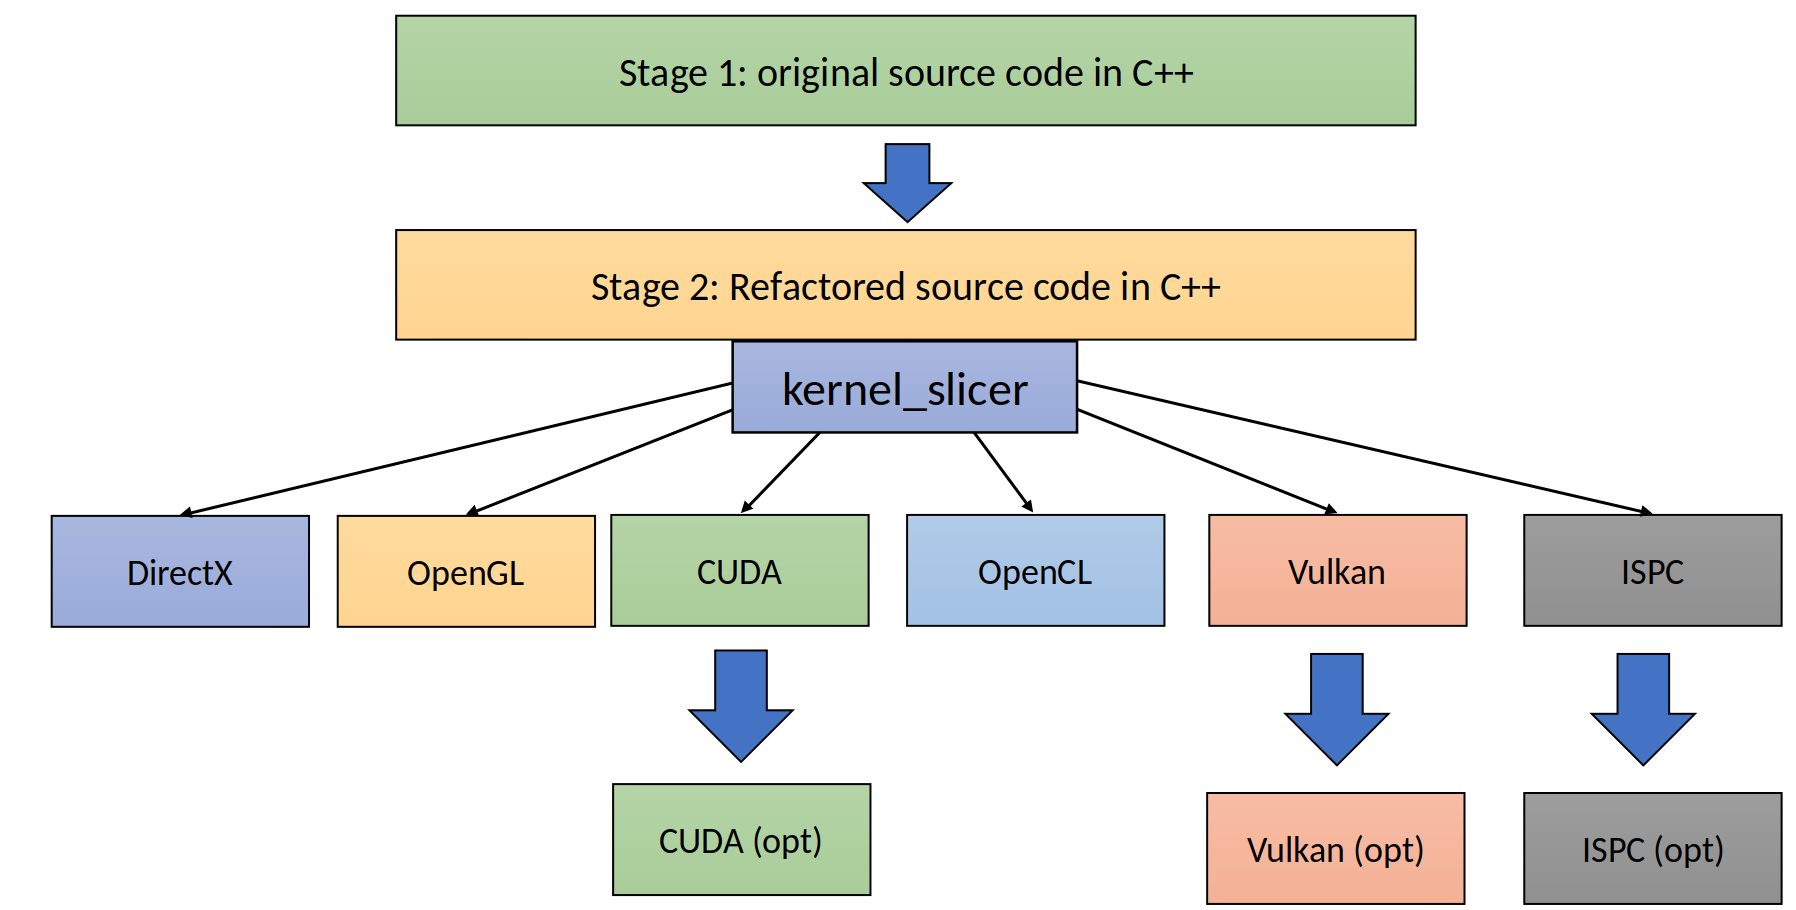
\includegraphics[width=0.5\textwidth]{kslicer_pipeline.jpg}
\caption{Концепция разработки с kernel\_slicer. На последнем шаге Вы можете самостоятельно доработать сгенерированный код на каком-то из существующиз API.}
\end{figure}

Такой механизм позволяет Вам добавить абсолютно любое изменение в Vulkan-код прозрачным способом. При этом Вы будете писать вручную на Vulkan лишь небольшую часть кода, которая обращается со специфическим аппаратным ускорением.

%\chapterimage{ice_rt.jpg} % Chapter heading image
%\chapter{Особенности паттерна трассировки лучей}\label{ray_tracing}


\chapterimage{shaman_vulkan_buben.jpg} % Chapter heading image
\chapter{Работа с Vulkan-интерфейсом напрямую}\label{vulkan-direct}

\chapterimage{velik.jpg} % Chapter heading image
\chapter{Работа с ISPC}

\chapterimage{literature.jpg} 

\begin{thebibliography}{10}
	
	\bibitem{NVCPP} NVIDIA. \textit{NVC++: a C++17 compiler for NVIDIA GPUs and AMD, Intel, OpenPOWER, and Arm CPUs.} // 	
	
	\bibitem{CUDA} NVIDIA, Vingelmann, P. \& Fitzek, F.H.P., 2020. CUDA, release: 10.2.89, Available at: https://developer.nvidia.com/cuda-toolkit.	
	
	\bibitem{OpenACC} ``OpenACC'', 2021 URL: https://www.openacc.org/
	
	\bibitem{ispc} Matt Pharr, William R. Mark. ``spc: A SPMD Compiler for High-Performance CPU Programming''
	
	\bibitem{Reinhard05} Reinhard, E., Ward, G., Pattanaik, S., and Debevec, P. \textit{High Dynamic Range Imaging: Acquisition, Display and Image-Based Lighting}, 2005.
	
	\bibitem{Mantiuk08} Mantiuk R., Daly S., Kerofsky L. Display adaptive tone mapping //ACM SIGGRAPH 2008 papers. – 2008. – С. 1-10.
	
	\bibitem{litert} Библиотека трассировки лучей, разрабатываемая в лаборатории компьютерной графики ВМК МГУ https://github.com/msu-graphics-group/CrossRT
	
	\bibitem{issue16} Рекурсивная поддержка функций с указателями \href{https://github.com/Ray-Tracing-Systems/kernel_slicer/issues/16}{https://github.com/Ray-Tracing-Systems/kernel\_slicer/issues/16}
	
\end{thebibliography}

\end{document}